\documentclass[a4paper,12pt,openright,titlepage,oneside]{book}

%\usepackage[english,brazil]{babel} 
%Define regra de gramática para separar síbalas {babel}
%e altera os títulos (como chapters, sections, references) para português
\usepackage[english]{babel}
\usepackage[hidelinks]{hyperref}
\usepackage{listings}
\usepackage{titletoc}
\usepackage{notoccite}
\usepackage{float}
\usepackage{algorithm}
%\usepackage[algo2e]{algorithm2e} 
\usepackage{arevmath}     % For math symbols
\usepackage[noend]{algpseudocode}
% Define uso de caracteres acentuados no PDF gerado
% e permite copiar corretamente o texto do PDF.
\usepackage[T1]{fontenc}
\usepackage[utf8]{inputenc}
\usepackage{booktabs}
\usepackage{mathtools}
\usepackage{amsmath}

\usepackage{appendix}

\makeatletter
\AtBeginDocument{\let\book@l@chapter\l@chapter}
\newcommand{\demotechaptersintoc}{%
  \addtocontents{toc}{\let\protect\l@chapter\protect\l@section}%
}
\newcommand{\promotechaptersintoc}{%
  \addtocontents{toc}{\let\protect\l@chapter\protect\book@l@chapter}%
}


\usepackage{doi}
% \usepackage[natbibapa]{apacite}
% Adição do pacote do template da UnB
\usepackage{template-FT-UnB/ft2unb}

\DeclareGraphicsExtensions{.jpg,.pdf,.mps,.png,.gif, .eps}
\graphicspath{imagens} %define diretório de imagens

%Arquivo com lista com hifenização correta de algumas palavras.
%Defina novas palavras no arquivo a medida que verificar que a hifenização automática
%etá errada para tais palavras.
%----------------DEFINE FORMA CORRETA DE HIFENIZAÇÃO PARA ALGUMAS PALAVRAS ----------------
\hyphenation{cons-tru-a}
\hyphenation{e-xem-plo}
\hyphenation{e-xem-plar}
\hyphenation{e-le-men-to}
\hyphenation{e-le-men-tar}
\hyphenation{ma-nu-al}
\hyphenation{res-pos-ta}
\hyphenation{ca-rac-te-ris-ti-ca}
\hyphenation{ca-rac-te-ris-ti-cas}
\hyphenation{ca-rac-te-ris-ti-co}
\hyphenation{ca-rac-te-ris-ti-cos}
\hyphenation{cor-res-pon-den-ci-as}
\hyphenation{cons-tru-am}
\hyphenation{re-a-li-za-da}
\hyphenation{re-a-li-za-do}
\hyphenation{re-a-li-za-das}
\hyphenation{re-a-li-za-dos}
\hyphenation{i-ne-xis-ten-cia}
\hyphenation{i-ne-xis-te}
\hyphenation{e-xis-te}
\hyphenation{di-fe-ren-te}
\hyphenation{di-fe-ren-tes}
\hyphenation{dei-xan-do}
\hyphenation{ins-ta-la-do} 
\hyphenation{ins-ta-la-dos} 
\hyphenation{ins-ta-la-da}
\hyphenation{ins-ta-la-das}
\hyphenation{re-gis-tra-do}
\hyphenation{re-gis-tra-dos}
\hyphenation{re-gis-tra-da}
\hyphenation{re-gis-tra-das}
\hyphenation{des-cre-ve}
\hyphenation{res-pei-to}
\hyphenation{re-a-li-za}
\hyphenation{re-a-li-zar}
\hyphenation{a-tu-a-li-zar}
\hyphenation{a-tu-a-li-zan-do}
\hyphenation{a-tu-a-li-za-do}
\hyphenation{a-tu-a-li-za-da}
\hyphenation{fun-ci-o-na-li-da-de}
\hyphenation{pos-si-bi-li-da-de}
\hyphenation{dis-po-si-ti-vo}
\hyphenation{dis-po-si-ti-vos}
\hyphenation{e-xis-te}
\hyphenation{e-xis-tir}
\hyphenation{des-co-ber-ta}
\hyphenation{des-co-ber-to}
\hyphenation{de-sig-nar}
\hyphenation{de-sig-na-do}
\hyphenation{o-pe-ra-ci-o-nais} 
\hyphenation{o-pe-ra-ci-o-nal}
\hyphenation{con-si-de-ra-do}
\hyphenation{con-si-de-ra-dos}
\hyphenation{ou-tro}
\hyphenation{ou-tra}
\hyphenation{ou-tros}
\hyphenation{ou-tras}
\hyphenation{e-xis-ten-te}
\hyphenation{e-xis-ten-tes}
\hyphenation{LuaOnTV}
\hyphenation{De-fi-ni-tion}
%------------------------------------------------------------------------------------------ 
\usepackage{xcolor}

% \newcommand*{\doi}[1]{\href{http://dx.doi.org/#1}{doi: #1}}
% \newcommand{\todo}[1]{\textcolor{red}{TODO: #1}\PackageWarning{TODO:}{#1!}}

% \usepackage[num,abnt-emphasize=bf,abnt-etal-text=it,abnt-doi=doi,bibjustif]%
% % ALTERE OS VALORES DENTRO DAS CHAVES DOS COMANDOS NESTA SEÇÃO PARA INCLUIR OS SEUS DADOS E DADOS DA SUA
% % DISSERTAÇÃO DE MESTRADO OU TESE DE DOUTORADO
% % -----------------------------------------------------------------------------------------------------
% }
%\onehalfspacing
\title{Framework for Object Detection and Distance Measurement on Self-Driving Cars using Multi-Cameras Perspective}

\author{BRUNO JUSTINO GARCIA PRACIANO}
\date{2019-07-16} %data da defesa

\grau{Mestre} %Mestre ou Doutor
\area{Sistemas Mecatrônicos} %Nome do curso
\siglaarea{ENM} %Sigla do departamento
\tipodemonografia{Dissertação} %Dissertação ou Tese
\programa{Mestrado} %Mestrado ou Doutorado
\autorendereco{} %Endereço do autor da dissertação/tese
\totalpgs{140} %total de páginas atualmente na sua dissertação
\dia{16} %dia da defesa
\mes{Julho} %mês da defesa
\ano{2019} %ano da defesa
\numpublicacao{150/2019} %número da publicação (após a defesa, tal número deve ser obtido na secretaria)

%PPGEE.DM  = Programa de Pós Graduação em ENgenharia Elétrica.Dissertação de Mestrado
%PPGENE.TD  = Programa de Pós Graduação em ENgenharia Elétrica.Tese de Doutorado
\siglapublicacao{PPMEC.TD}

\titulolinhai{Framework for Object Detection and Distance }
\titulolinhaii{Measurement on Self-Driving Cars}
\titulolinhaiii{using Multi-Cameras Perspective}

\autori{BRUNO JUSTINO GARCIA PRACIANO}
%Caso seu nome não caiba em uma única linha, divida ele nos comandos abaixo
%\autorii{} 
%\autoriii{}

\membrodabancai{Prof. Dr.-Ing João Paulo Carvalho Lustosa da Costa, ENE/UnB}
\membrodabancaifuncao{Membro Interno - Presidente}

\membrodabancaii{Prof. Dr. Rafael T. de Sousa Jr., ENE/UnB}
\membrodabancaiifuncao{Examinador Interno}

\membrodabancaiii{Prof. Dr. Robson de Oliveira Albuquerque, CEPESC}
\membrodabancaiiifuncao{Examinador Externo}




% -----------------------------------------------------------------------------------------------------

%line-numbers, inputencoding=utf8/latin1
%Define o estilo para listagens de código fonte
\lstset{
  numbers=left, %numeração de linhas à esquerda
  stepnumber=1,
  firstnumber=1,
  numberstyle=\tiny,
  extendedchars=true,
  frame=none,
  basicstyle=\footnotesize,
  stringstyle=\ttfamily,
  showstringspaces=false,
  %language=Java, %deve ser definida na inclusão de cada trecho de código, pois podem existir linguagens diferentes em exemplos diferentes
  breaklines=true,
  breakautoindent=true,
  %estilos de comentário de uma e várias linhas
  morecomment=[l]{--}, morecomment=[s]{/*}{*/}, morecomment=[s]{<!--}{-->}, morecomment=[s]{--[[}{--]]}
}

% Adição de metadados no PDF (propriedades do documento PDF)
\makeatletter
	 \hypersetup{
		 pdftoolbar=true,        % show Acrobat’s toolbar?
		 pdfmenubar=true,        % show Acrobat’s menu?
		 pdffitwindow=false,     % window fit to page when opened
		 pdfstartview={FitH},    % fits the width of the page to the window	 
		 pdftitle={\@title},
		 pdfauthor={\@author},
		 pdfsubject={\tipodemonografianome \ de\ \programastr \ em\ \areastr},   % subject of the document
		 pdfcreationdate={\pdfdate}
	 }
\makeatother


\makeindex
\makenomenclature %Necessário para gerar lista de siglas


\begin{document}

	\pdfbookmark[0]{Agradecimentos}{agradecimentos}
	%* indica para nao adicionar numeracao ao titulo
\chapter*{Acknowledgments}

First of all, I would like to thank God for giving me health and concentration during the COVID19 crises in Europe and for not allowing anything bad to happen with me.

Also, I leave my immense gratitude for the University of Brasilia for the acquired knowledge along these years.


I am eternally thankful to my family Alessandra Justino, Flávio Praciano, Lenita Justino, and Victor Hugo, whom I can count and trust unconditionally.

An invaluable character is my master tutor Prof. Dr.-Ing. Joao Paulo C. L da Costa, who directed me to the new field of autonomous vehicles, and for always motivate me to do my best.

I would like to demonstrate my gratitude for my advisor Lothar Weichenberger for trust in my work and always support me and a special thanks for the company Elektronische Fahrwerksystem GmbH for financial and structural support. Another very essential characters in my thesis are Lukac Branimir, Tobias Behn, and Andreas Schustek without their valuable support it would not possible to do much of my work.

Along this road, I had some problems with german bureaucracy, my sincere thanks for Lukas Bös for his unbelievable capacity to solve problems and his communication skills, also I need to thank Sara Martin and Robin Käsmayr for their support and also students who attended our Stammtisch. And Vanessa Voll for all the help provided.

I would like to thanks the lunch clubs of Latino brothers composed by Javier Rivas, Arnaldo Arancíbia, Gabriel Pinheiro, João Paulo, and me for the good conversations and for supporting me to improve my Spanish while I was living in Germany.

My time in Germany was excellent due to the great hospitality of my host family, my thankful to Johanna Hirschmann and Herbert Hirschmann for made it easy everything. 

Additionally, his unconditional helpfulness and psychological support were simply
crucial, my friends were very important, in special my flatmate Gabriel Pinheiro, Lucas Maciel, Yan Trindade, Fábio Mendonça, Daniel Alves, Francisco Lopes, Robson de Albuquerque, and Rafael Timoteo. 

I also express my sincere gratitude for the professors from the University of Brasilia in special for Prof.Dr. Rafael Timoteo de Sousa Junior for his invaluable support and his guidance along with my career. And for prof. Dr. Edna Canedo, prof. Dr. Georges Amvame for partnership in some papers publications.

My sincere gratitude for the Institutional Security Office of the Presidency of the Republic of Brazil (Grant 002/2017) and to FAPDF (Projetos UIoT 0193.001366/2016) whose I have a scholarship and supported me to pay the conference fees. 
	\begin{flushright}
\chapter*{Resumo}
\end{flushright}

\noindent
Neste trabalho é realizada a proposta de um sistema multicameras para detecção de objetos, e também a medição da distância através de visão computacional. Avalia-se o desempenho de outras técnicas para levar em consideração o melhor resultado do framework proposto. Uma vez implementados os algoritmos, existem diversos outros cenários e caractéristicas que podem ser levadas em consideração para um possível erro de medição da distância, na maioria das vezes esse erro está diretamente relacionado a fatores meteriológicos e também a sinal fraco de comunicação entre as câmeras e o hardware de controle. Através dos resultados obtidos, percebe-se que em condições ideias e em ambientes controlados, os métodos de detecção de objetos garatem precisão satisfatória, com a acurácia acima de 93\%, mas quando existe outro objeto em frente a ele, a acurácia reduz drásticamente. Para reduzir esses problemas, foi proposto a otimização do posicionamento das câmeras, assim como o ângulo de inclinação. 


\noindent
Palavras-chave: \textbf{Veículos autônomos; Visão computacional; Detecção de objetos; Estimação de distância}.




	\begin{flushright}
\chapter*{Abstract}
\end{flushright}

\noindent
In this work, a proposal is made for a multicamera system for object detection, as well as distance measurement through computer vision. The performance of other techniques is evaluated to take into account the best result of the proposed framework. Once the algorithms have been implemented, there are several other scenarios and characteristics that can be taken into account for a possible distance measurement error, most of the time this error is directly related to meteorological factors and also to a weak communication signal between cameras and the control hardware. Through the results obtained, it is noticed that in ideal conditions and in controlled environments, the methods of object detection guarantee satisfactory precision, with an accuracy above 93 \%, but when there is another object in front of it, the accuracy drastically reduces . To reduce these problems, it was proposed to optimize the positioning of the cameras, as well as the angle of inclination.


\noindent
Keywords: \textbf{Autonomous Vehicles; Computional Vision; Object Detection; Distance Estimation}.
	\pdfbookmark[0]{Sumário}{sumario}
	\sumario
	
	\pdfbookmark[0]{List of Figures}{listafiguras}
	\listadefiguras
	
	\pdfbookmark[0]{List of Tables}{listatabelas}
	\listadetabelas
	
% 	\pdfbookmark[0]{Lista de Códigos Fonte}{listacodigosfonte}
% 	\listadecodigosfonte
	
	\renewcommand{\nomname}{ACRONYMS} %Define um caption à lista de siglas
	%Inclui a lista de siglas 
% 	\pdfbookmark[0]{ACRONYMS}{nomenclatura}
	
% 	\nomenclature{IoT}{Internet of Things}
% 	\nomenclature{RNP}{Rede Nacional de Ensino e Pesquisa}
% 	\nomenclature{P2P}{\textit{Peer-to-Peer} (Ponto a Ponto)}
% 	\nomenclature{IaaS}{\textit{Infrastructure as a Service}}
% 	\nomenclature{IDE}{\textit{Integrated Development Environment}}
% 	\nomenclature{IP}{\textit{Internet Protocol Version 4}}
% 	\nomenclature{IPv6}{\textit{Internet Protocol Version 6}}
% 	\nomenclature{JSON}{\textit{JavaScript Object Notation}}
% 	\nomenclature{REST}{\textit{Representational State Transfer}}
% 	\nomenclature{RFID}{\textit{Radio Frequency identification}}
% 	\nomenclature{SQL}{\textit{Structured Query Language}}
% 	\nomenclature{TCP}{\textit{Transmission Control Protocol}}
% 	\nomenclature{API}{\textit{Application Programming Interface}}
% 	\nomenclature{WSN}{\textit{Wireless Sensor Networks}}
% 	\nomenclature{UUID}{\textit{Universal Unique Identifier}}
% 	\nomenclature{GPS}{\textit{Global Positioning System}}
%     \nomenclature{LPS}{\textit{Local Positioning System}}
%     \nomenclature{DDS}{\textit{Distributed data service}}
% 	\nomenclature{SOA}{\textit{Service Oriented Architecture}}
% 	\nomenclature{VM}{\textit{Virtual Machine}}
% 	\nomenclature{IEEE}{Institute of Electrical and Electronics Engineers}
	

	
	\printnomenclature[2.5cm] 
	\mainmatter %Inicia a numeracao normal cardinal
	\setcounter{page}{1} \pagenumbering{arabic} \pagestyle{plain}
	
	\chapter{Introduction} \label{introducao}
The research area of autonomous vehicles (AV) is totally multidisciplinary, with the way the vehicle is built, it is possible to create high impact applications, which establish interrelations and information flows and detect new extended stimuli in scenarios where the infrastructure is physical or mobile \cite{bayat2017environmental}. With this, there is the possibility to apply the concepts of computer vision, which allows the car to see the external environment and combined with Machine Learning (ML) tools the vehicle begins to interpret what is around it \cite{rasouli2019autonomous}.

One of the major challenges of AV is detect the position of the car along the road, it is possible to perform this task using vehicle to infrastructure (V2I), or with other technique such as GPS \cite{hobert2015enhancements}. Therefore, there are some studies to investigate the acceptation of the AV and a way to proof this new technology can reduce the car accidents, as study guided by Xu et. al where Of the respondents, 42.35\% and 45.28\% expect lower risk and lower insurance premiums for autonomous vehicles, respectively \cite{xu2019autonomous}.

Considering that it is possible to have cameras around the road, in this thesis, we propose an object detection model using multi-cameras, where there is a responsible algorithm for detecting and classifying objects, as well as estimating the distance where that object is positioned.

\section{Motivation}

The autonomous vehicles are the new reality for the next years with this premise, the new solutions need to grow, and one of these important necessities is the vehicle tracking, and should reduce the traffic jams and decrease the number of cars crash \cite{bonnefon2016social}. Given that, there are many levels of self-drive car automation as shown in Figure \ref{fig:automation}. This work is focused on the test scenario of driving automation. Due to drones requires much battery during the test and limits the scenario to 30 to 45 minutes, the proposal is to use the infrastructure along the road as a camera on the pole and send the data to a command center.

\begin{figure}[H]
\centering
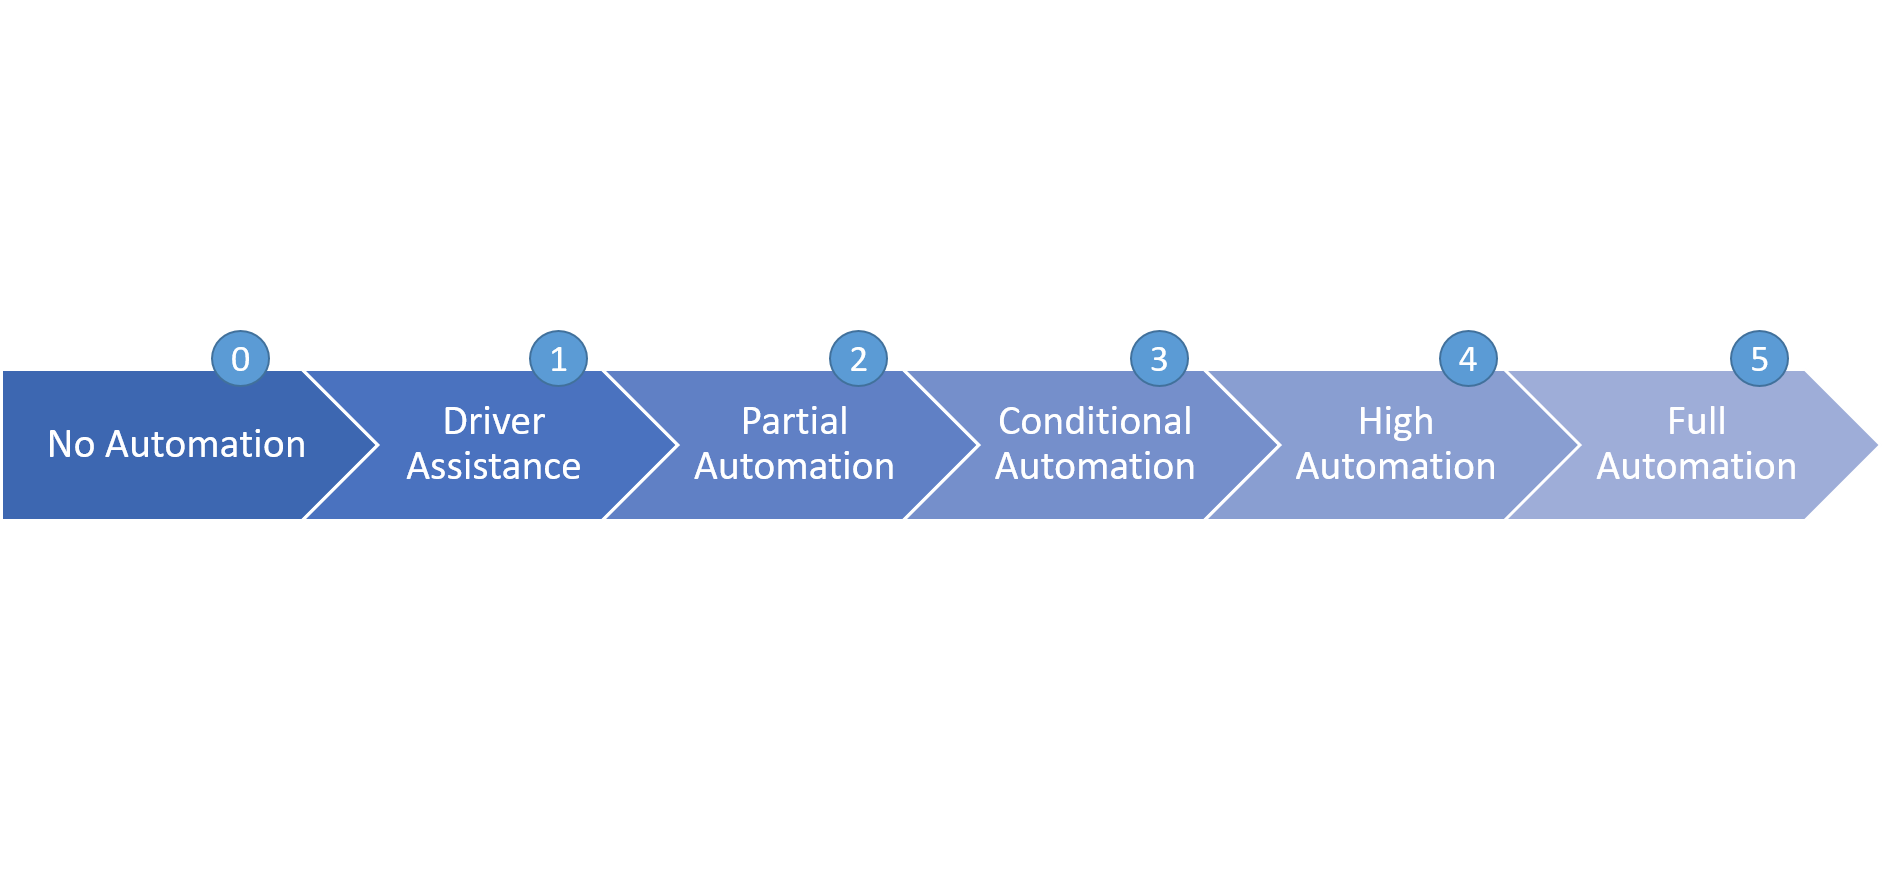
\includegraphics[scale=0.55]{imagens/diagrama_levels.png}
\caption{Levels of driving automation}
\label{fig:automation}
\end{figure}

\section{Problem Description}

The problem of this theme is to create an architecture to detect objects along the roads combined with the distance measurement of these along the road. The first approach could be using a drone, but due to the battery conditions for long tests, it is not a good choice. Figure \ref{fig:tests} shown this problem. The goal is to track the position of the cars even vehicles under the test (VUT) and traffic simulation data (TSV) along the road and send this information to the command central (CC). 

\begin{figure}[H]
\centering
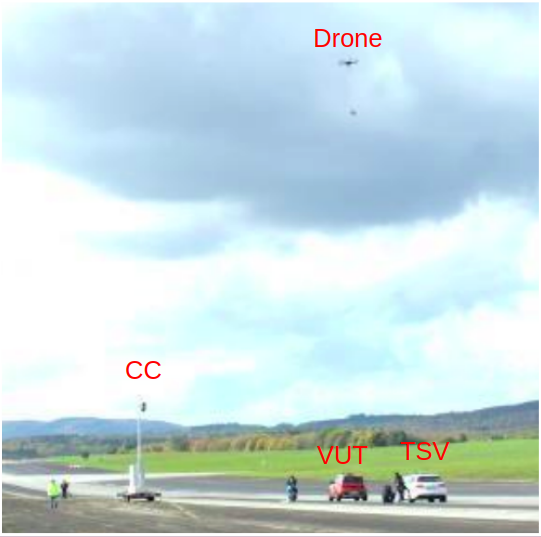
\includegraphics[scale=0.6]{imagens/proposal.png}
\caption{Modelling of the project using drones, where CC means command central, VUT is vehicle under the tests and TSV is traffic simulation vehicle.}
\label{fig:tests}
\end{figure}

\section{Objectives}

Create a framework able to detect objects as cars, trucks, motorcycles, pedestrians, and other strange obstacles along the road, and with these capacities estimate the distance of this object along the road, this framework is necessary to work with a camera array.

\section{Published Works}

Along with the development of this work, the author worked in several areas of computer sciences, in special data science domain, and always trying to keep the multidisciplinarity. These are my published works along my master degree:

\begin{enumerate}

\item \textbf{PRACIANO, BRUNO J. G.}; DE CALDAS FILHO, FRANCISCO L. ; E MARTINS, LUCAS M. C. ; DA CUNHA, DAYANNE F. ; DA SILVA, DANIEL ALVES ; DE SOUSA JÚNIOR, RAFAEL TIMÓTEO. SEGURANÇA DO AMBIENTE USANDO DISPOSITIVO IOT COM PROCESSAMENTO DISTRIBUÍDO. In: Atas da conferência IberoAmericana WWW/Internet 2019, 2019. Atas da conferência Ibero-Americana WWW/Internet 2019, 2019. p. 163

\item MARQUES, Angelica Alves da Cunha; \textbf{PRACIANO, Bruno Justino Garcia}. Researchers of the Brazilian archivistics scientific community in French international areas of interlocution Encontros Bibli: revista eletrônica de biblioteconomia e ciência da informação, Florianópolis, v. 25, p. 01-14, mar. 2020. ISSN 1518-2924. doi:https://doi.org/10.5007/1518-2924.2020.e65864.

\item CASTELINO, R. M.; MOREIRA, G. P.; \textbf{PRACIANO, BRUNO JUSTINO GARCIA} ; SANTOS, GIOVANNI A.; WEICHENBERGER, L.; DE SOUSA, JR, RAFAEL T. Improving the accuracy of pedestrian detection in partially occluded or obstructed scenarios. In: 2020 10th International Conference on Advanced Computer Information Technologies, 2020, Deggendorf. 2020 10th International Conference on Advanced Computer Information Technologies, 2020. (to be published)

\item CANEDO, EDNA; PINHEIRO, GABRIEL; SOUSA JR., RAFAEL; RIBEIRO, RENATO; \textbf{PRACIANO, BRUNO} ; LOPES DE MENDONÇA, FÁBIO. Front End Application Security: Proposal for a New Approach. In: 22nd International Conference on Enterprise Information Systems, 2020, Prague. Proceedings of the 22nd International Conference on Enterprise Information Systems, 2020. p. 233.

\item SOUSA JR., RAFAEL; LOPES DE MENDONÇA, FÁBIO; NZE, GEORGES; PINHEIRO, GABRIEL; \textbf{PRACIANO, BRUNO }; CANEDO, EDNA. Performance Evaluation of Software Defined Network Controllers. In: 10th International Conference on Cloud Computing and Services Science, 2020, Prague. Proceedings of the 10th International Conference on Cloud Computing and Services Science, 2020. p. 363.


\item SILVA, DANIEL ALVES DA; TORRES, JOSÉ ALBERTO SOUSA; PINHEIRO, ALEXANDRE; DE CALDAS FILHO, FRANCISCO L.; MENDONÇA, FABIO L. L.; \textbf{PRACIANO, BRUNO J. G} ; KFOURI, GUILHERME OLIVEIRA; DE SOUSA, JR, RAFAEL T. Inference of driver behavior using correlated IoT data from the vehicle telemetry and the driver mobile phone. In: 2019 Federated Conference on Computer Science and Information Systems, 2019. org.crossref.xschema.\_1.Title@7d70270b, 2019. p. 487.

\item KFOURI, GUILHERME DE O. ; GONÇALVES, DANIEL G. V. ; DUTRA, BRUNO V. ; ALENCASTRO, JOÃO F. DE ; FILHO, FRANCISCO L. DE CALDAS ; MARTINS, LUCAS M. C. E ; \textbf{PRACIANO, BRUNO J. G.} ; ALBUQUERQUE, ROBSON DE O. ; JR, RAFAEL T. DE SOUSA . Design of a Distributed HIDS for IoT Backbone Components. In: 2019 Federated Conference on Computer Science and Information Systems, 2019. org.crossref.xschema.\_1.Title@7bad8b1f, 2019. p. 81.

\item DE MENDONCA, FABIO L. L.; DA CUNHA, DAYANNE F.; \textbf{PRACIANO, BRUNO J. G.} ; DA ROSA ZANATTA, MATEUS; DA COSTA, JOAO PAULO C. L.; DE SOUSA, RAFAEL T. P2PIoT: A Peer-To-Peer Communication Model for the Internet of Things. In: 2019 Workshop on Communication Networks and Power Systems (WCNPS), 2019, Brasilia. 2019 Workshop on Communication Networks and Power Systems (WCNPS), 2019. p. 1.

\item BRANDAO, IURE V.; DA COSTA, JOAO PAULO C. L.; SANTOS, GIOVANNI A.; \textbf{PRACIANO, BRUNO J}. G.; JUNIOR, FRANCISCO C. M. D.; DE S. JUNIOR, RAFAEL T. Classification and predictive analysis of educational data to improve the quality of distance learning courses. In: 2019 Workshop on Communication Networks and Power Systems (WCNPS), 2019, Brasilia. 2019 Workshop on Communication Networks and Power Systems (WCNPS), 2019. p. 1.


\item DO NASCIMENTO SILVA, GERSON ; DE CALDAS FILHO, FRANCISCO LOPES ; DOS REIS, VINICIUS ELOY ; \textbf{PRACIANO, BRUNO JUSTINO }; LUSTOSA, JOÃO PAULO ; DE SOUSA JÚNIOR, RAFAEL TIMÓTEO . MODELO DE REDES NEURAIS ARTIFICIAIS EM SUPORTE TECNOLÓGICO À DETECÇÃO DE CARTEIS EM LICITAÇÕES PÚBLICAS. In: Atas da conferência IberoAmericana WWW/Internet 2019, 2019. Atas da conferência Ibero-Americana WWW/Internet 2019. p. 191.

\end{enumerate}

\section{Chapters Description}

This work is divided as follows: in Chapter 2, the state of the art will be presented, to support this work, once it is necessary to get a good part of the previous contributions in this research area. In Chapter 3, the theoretical concepts to support the understanding of this work will be presented, since self-drive cars are a new trend topic is necessary to describe step by step about this necessary to provide a good theoretical background. In Chapter 4, the proposed framework is shown and mathematical modeling is provided. In Chapter 5, the results will be discussed around the algorithm performance and the error for object detection position estimation. Finally, in Chapter 6, the conclusions will be discussed regarding the experiments, and some future works will be shown.



	\chapter{State of the art} \label{capitulo2}

The authors from the paper \cite{Lategahn2013} have presented the next generation driver assistance systems require precise self localization. Common approaches using global navigation satellite systems (GNSSs) suffer from multipath and shadowing effects often rendering this solution insufficient. In urban environments this problem becomes even more pro- nounced. Herein we present a system for six degrees of freedom (DOF) ego localization using a mono camera and an inertial measure- ment unit (IMU). The camera image is processed to yield a rough position estimate using a previously computed landmark map. Thereafter IMU measurements are fused with the position estimate for a refined localization update. Moreover, the mapping pipeline required for the creation of landmark maps. The accuracy of the system is evaluated by computing two independent ego positions of the same trajectory from two distinct cameras and investigating these estimates for consistency. A mean localization accuracy of 10 cm is achieved on a 10 km sequence in in an inner city scenario.

Video cameras are among the most commonly used sensors in a large number of applications, ranging from surveillance to smart rooms for videoconferencing. There is a need to develop algorithms for tasks such as detection, tracking, and recognition of objects, specifically using distributed networks of cameras. The projective nature of imaging sensors provides ample challenges for data association across cameras. We first discuss the nature of these challenges in the context of visual sensor networks. Then, we show how real-world constraints can be favorably exploited in order to tackle these challenges. Examples of real-world constraints are a) the presence of a world plane, b) the presence of a three-dimiensional scene model, c) consistency of motion across cameras, and d) color and texture properties. In this regard, the main focus of this paper is towards highlightingthe efficient use of the geometric constraints induced by the imaging devices to derive distributed algorithms for target detection, tracking, and recognition. Our discussions are supported by several examples drawn from real applications. Lastly, we also describe several potential research problems that remain to be addressed \cite{Sankaranarayanan2008}.

Commercial Unmanned aerial vehicle (UAV) industry, which is publicly known as drone, has seen a tremendous increase in last few years, making these devices highly accessible to public. This phenomenon has immediately raised security concerns due to fact that these devices can intentionally or unintentionally cause serious hazards. In order to protect critical locations, the academia and industry have proposed several solutions in recent years. Computer vision is extensively used to detect drones autonomously compared to other proposed solutions such as RADAR, acoustics and RF signal analysis thanks to its robustness. Among these computer vision-based approaches, we see the preference of deep learning algorithms thanks to their effectiveness. In this paper, we are presenting an autonomous drone detection and tracking system which uses a static wide-angle camera and a lower-angle camera mounted on a rotating turret. In order to use memory and time efficiently, we propose a combined multi-frame deep learning detection technique, where the frame coming from the zoomed camera on the turret is overlaid on the wide-angle static camera’s frame. With this approach, we are able to build an efficient pipeline where the initial detection of small sized aerial intruders on the main image plane and their detection on the zoomed image plane is performed simultaneously, minimizing the cost of resource exhaustive detection algorithm. In addition to this, we present the integral system including tracking algorithms, deep learning classification architectures and the protocols \cite{Unlu2019}.


With the three-dimensional (3D) coordinates of objects captured by a sequence of images taken in different views, object reconstruction is a technique which aims to recover the shape and appearance information of objects. Although great progress in object reconstruction has been made over the past few years, object reconstruction in occlusion situations remains a challenging problem. In this paper, we propose a novel method to reconstruct occluded objects based on synthetic aperture imaging. Unlike most existing methods, which either assume that there is no occlusion in the scene or remove the occlusion from the reconstructed result, our method uses the characteristics of synthetic aperture imaging that can effectively reduce the influence of occlusion to reconstruct the scene with occlusion. The proposed method labels occlusion pixels according to variance and reconstructs the 3D point cloud based on synthetic aperture imaging. Accuracies of the point cloud are tested by calculating the spatial difference between occlusion and non-occlusion conditions. The experiment results show that the proposed method can handle the occluded situation well and demonstrates a promising performance \cite{Pei2019}.

The focus of this paper is inter-vehicles distance measurement which is a very important and challenging task in image processing domain. Where it is used in several systems such as Driving Safety Support Systems (DSSS), autonomous driving and traffic mobility. In the current paper, we propose an inter-vehicle distance measurement system for self-driving based on image processing. The proposed system uses two cameras mounted as one stereo camera, in the hosting vehicle behind the rear-view mirror. The detection of vehicles is performed first in a single camera using a recent powerful work from the literature. Then, the same vehicle is detected in the image captured by the second camera using template matching technique. Thus, the inter-vehicle distance is calculated using a simple method based on the position of the vehicle in both cameras, geometric derivations and additional technical data such as distance between the cameras and some other specific angles (e.g. the cameras view field angle). The results of the extensive experiments showed the high accuracy of the proposed method compared to the previous works from literature and it allows to measure efficiently the distances between the vehicles and the hosting vehicle. In addition, this method could be used in several systems of various domains in real time regardless of the object types. The experiments results were done on a Hardware Processor System (HPS) located in a VEEK-MT2S provided by TERASIC \cite{Zaarane2020}.

Computer-vision methods have been extensively used in intelligent transportation systems for vehicle detection. However, the detection of severely occluded or partially observed vehicles due to the limited camera fields of view remains a challenge. This paper presents a multi-camera vehicle detection system that significantly improves the detection performance under occlusion conditions. The key elements of the proposed method include a novel multi-view region proposal network that localizes the candidate vehicles on the ground plane. We also infer the vehicle position on the ground plane by leveraging multi-view cross-camera context. Experiments are conducted on dataset captured from a roadway in Richardson, TX, USA, and the system attains 0.7849 Average Precision and 0.7089 Multi Object Detection Precision. The proposed system results in an approximately 31.2\% increase in AP and 8.6\% in MODP than the single-camera methods \cite{Wu2019}.

This paper describes systematically two methods used in intelligent transportation systems: Distance Estimation using an onboard camera and car position detection. Distance estimation is a method for detecting distance for the preceding vehicles based on monocular camera. Vehicle position detection is a method of specifying the vehicle position relative to the road that can serve as Lane Departure Warning system. These two approaches have been discussed and implemented in this article. For lane detection and tracking, Hough Transform and Kalman filter were adopted. A brief introduction about both lane detection system and object detection is given. Finally, both approaches have been evaluated on a large dataset of videos \cite{Ali2016}.

Cameras are a crucial exteroceptive sensor for self-driving cars as they are low-cost and small, provide appearance information about the environment, and work in various weather conditions. They can be used for multiple purposes such as visual navigation and obstacle detection. We can use a surround multi-camera system to cover the full 360-degree field-of-view around the car. In this way, we avoid blind spots which can otherwise lead to accidents. To minimize the number of cameras needed for surround perception, we utilize fisheye cameras. Consequently, standard vision pipelines for 3D mapping, visual localization, obstacle detection, etc. need to be adapted to take full advantage of the availability of multiple cameras rather than treat each camera individually. In addition, processing of fisheye images has to be supported. In this paper, we describe the camera calibration and subsequent processing pipeline for multi-fisheye-camera systems developed as part of the V-Charge project. This project seeks to enable automated valet parking for self-driving cars. Our pipeline is able to precisely calibrate multi-camera systems, build sparse 3D maps for visual navigation, visually localize the car with respect to these maps, generate accurate dense maps, as well as detect obstacles based on real-time depth map extraction \cite{Hane2017}.

We present a real-time dense geometric mapping algorithm for large-scale environments. Unlike existing methods which use pinhole cameras, our implementation is based on fisheye cameras whose large field of view benefits various computer vision applications for self-driving vehicles such as visual-inertial odometry, visual localization, and object detection. Our algorithm runs on in-vehicle PCs at approximately 15 Hz, enabling vision-only 3D scene perception for self-driving vehicles. For each synchronized set of images captured by multiple cameras, we first compute a depth map for a reference camera using plane-sweeping stereo. To maintain both accuracy and efficiency, while accounting for the fact that fisheye images have a lower angular resolution, we recover the depths using multiple image resolutions. We adopt the fast object detection framework, YOLOv3, to remove potentially dynamic objects. At the end of the pipeline, we fuse the fisheye depth images into the truncated signed distance function (TSDF) volume to obtain a 3D map. We evaluate our method on large-scale urban datasets, and results show that our method works well in complex dynamic environments \cite{Cui2019}.

Advanced driver assistance systems (ADAS) based on monocular vision are rapidly becoming a popular research subject. In ADAS, inter-vehicle distance estimation from an in-car camera based on monocular vision is critical. At present, related methods based on a monocular vision for measuring the absolute distance of vehicles ahead experience accuracy problems in terms of the ranging result, which is low, and the deviation of the ranging result between different types of vehicles, which is large and easily affected by a change in the attitude angle. To improve the robustness of a distance estimation system, an improved method for estimating the distance of a monocular vision vehicle based on the detection and segmentation of the target vehicle is proposed in this paper to address the vehicle attitude angle problem. The angle regression model (ARN) is used to obtain the attitude angle information of the target vehicle. The dimension estimation network determines the actual dimensions of the target vehicle. Then, a 2D base vector geometric model is designed in accordance with the image analytic geometric principle to accurately recover the back area of the target vehicle. Lastly, area-distance modeling based on the principle of camera projection is performed to estimate distance. The experimental results on the real-world computer vision benchmark, KITTI, indicate that our approach achieves superior performance compared with other existing published methods for different types of vehicles (including front and sideway vehicles) \cite{Huang2019}.

Self-localization is one of the most important part in autonomous driving system. In urban canyon, the multipath and non-line-of-sight effects to GPS receiver decrease the precision of self-localization of the vehicle. More specifically, the lateral error is more serious because of the blockage of the satellites. However, the building on roadside could be the stable reference object for localization. Therefore, this paper proposes to use stereo camera and 3D building map to reduce the lateral error of positioning result. In our proposal, stereo camera is used to detect and reconstruct the building side view. Lateral distance between building and vehicle estimated by stereo camera is compared with 3D building map to rectify the lateral position of vehicle. In addition, this paper employs inertial sensor and GPS receiver to decide the longitudinal position of vehicle. The particle filter is used for the sensor fusion. The experiment is conducted in the center of Tokyo, Japan, which is a typical urban city scene with high density of tall buildings. It demonstrates that the proposed method could achieve sub-meter level accuracy in GPS difficult environments \cite{Bao2016}.

Urban traffic optimization using traffic cameras as sensors is driving the need to advance state-of-the-art multi-target multi-camera (MTMC) tracking. This work introduces CityFlow, a city-scale traffic camera dataset consisting of more than 3 hours of synchronized HD videos from 40 cameras across 10 intersections, with the longest distance between two simultaneous cameras being 2.5 km. To the best of our knowledge, CityFlow is the largest-scale dataset in terms of spatial coverage and the number of cameras/videos in an urban environment. The dataset contains more than 200K annotated bounding boxes covering a wide range of scenes, viewing angles, vehicle models, and urban traffic flow conditions. Camera geometry and calibration information are provided to aid spatio-temporal analysis. In addition, a subset of the benchmark is made available for the task of image-based vehicle re-identification (ReID). We conducted an extensive experimental evaluation of baselines/state-of-the-art approaches in MTMC tracking, multi-target single-camera (MTSC) tracking, object detection, and image-based ReID on this dataset, analyzing the impact of different network architectures, loss functions, spatio-temporal models and their combinations on task effectiveness. An evaluation server is launched with the release of our benchmark at the 2019 AI City Challenge (https://www.aicitychallenge.org/) that allows researchers to compare the performance of their newest techniques. We expect this dataset to catalyze research in this field, propel the state-of-the-art forward, and lead to deployed traffic optimization(s) in the real world \cite{Tang2019}.

In order to measure the distance between our vehicle and the target vehicle by monocular vision and eliminate the estimation error bring by changing of vehicle pose, we propose the distance estimation method based on the vehicle pose information, which can be used to eliminate the error of distance estimation effectively cause by the change of the pitch angle and roll angle of unmanned vehicle. In addition, the pose information could also help us estimate whether the vehicle is in a slope, thus engage in distance estimation for the vehicles. Several groups of data was collected for the experiments. And the result prove the validity of the algorithm in distance estimation \cite{Qi2019}.

This paper presents a distance determination technique using an image from the single forward camera. Since too dark or too bright of the image and non-linear relation between height of the object and distance from the camera have effect on the performance of the detection process. Therefore, automatic brightness adjustment and inverse perspective mapping (IMP) is applied in the proposed scheme. In addition, region of interest (ROI) determination is used to decrease the processing time. The experimental results confirm that the proposed technique can detect distance of the object in front of the car where the error is 7.96\% \cite{Wongsaree2018}.

Global calibration of multi-vision sensors in the railway fields is easily affected by on-site complex environments, such as lighting and self-occlusion, which makes it difficult for existing methods to achieve high-Accuracy calibration. In this paper, a high-Accuracy and flexible calibration method of multi-vision sensors in the outdoor railway fields based on flexible and optimal 3D data field through the combination of articular arm and metal target embedded with luminescent LEDs is proposed. Firstly, a high-Accuracy and flexible 3D data field with multiple angles and views is constructed by the articular arm and the metal target rapidly; Secondly, the high-frequency multi-exposure imaging mode and multi-scale image feature points extraction are adopted, and the high-Accuracy reposition is achieved through Kalman filter, which can reduce the impact of image noise efficiently; Finally, the RANSAC method is utilized to optimize the 3D data field, forming the optimal 3D data field, and the optimal target chains corresponding to each group of cameras are established. The maximum likelihood solution of global parameters is solved by nonlinear optimization. Simulation experiments verify the feasibility of the proposed method. Meanwhile, physical experiment results show this method can reduce the outdoor environment impact and improve the calibration and measurement precision effectively. In addition, the computational efficiency of the proposed method is about 11.2 times than multi-images averaging method, the calibration and measurement accuracy improve about 20 and 2.9 times respectively, which is suitable for the high-Accuracy and flexible global calibration in the complex railway environment \cite{Pan2019}.

This paper presents a novel method of camera parameters calibration for obstacle distance measurement based on monocular vision. In this method, resolving camera parameters have been decomposed into two linear equation sets, which has significantly reduced computing complexity and improved computing speed. The ideal pinhole imaging model of obstacle has been demonstrated, then the linear equations have been derived afterwards. In the end, experiment shows that the proposed method is very effective \cite{Lin2014}.

Accurate detection of 3D objects is a fundamental problem in computer vision and has an enormous impact on autonomous cars, augmented/virtual reality and many applications in robotics. In this work we present a novel fusion of neural network based state-of-the-art 3D detector and visual semantic segmentation in the context of autonomous driving. Additionally, we introduce Scale-Rotation-Translation score (SRTs), a fast and highly parameterizable evaluation metric for comparison of object detections, which speeds up our inference time up to 20\% and halves training time. On top, we apply state-of-the-art online multi target feature tracking on the object measurements to further increase accuracy and robustness utilizing temporal information. Our experiments on KITTI show that we achieve same results as state-of-the-art in all related categories, while maintaining the performance and accuracy trade-off and still run in real-time. Furthermore, our model is the first one that fuses visual semantic with 3D object detection \cite{Simon2019a}.

In this paper, we propose weighted-mean YOLO to improve real-time performance of object detection by fusing information of RGB camera and LIDAR. RGB camera is vulnerable to external environments and therefore strongly affected by illumination. Conversely, LIDAR is robust to external environments, but has low resolution. Since each sensor can complement their disadvantages, we propose a method to improve the performance of object detection through sensor fusion. We design the system using weighted-mean to construct a robust system and compared with other algorithms, it shows performance improvement of missed-detection \cite{Kim2019}.

Lidar based 3D object detection is inevitable for autonomous driving, because it directly links to environmental understanding and therefore builds the base for prediction and motion planning. The capacity of inferencing highly sparse 3D data in real-time is an ill-posed problem for lots of other application areas besides automated vehicles, e.g. augmented reality, personal robotics or industrial automation. We introduce Complex-YOLO, a state of the art real-time 3D object detection network on point clouds only. In this work, we describe a network that expands YOLOv2, a fast 2D standard object detector for RGB images, by a specific complex regression strategy to estimate multi-class 3D boxes in Cartesian space. Thus, we propose a specific Euler-Region-Proposal Network (E-RPN) to estimate the pose of the object by adding an imaginary and a real fraction to the regression network. This ends up in a closed complex space and avoids singularities, which occur by single angle estimations. The E-RPN supports to generalize well during training. Our experiments on the KITTI benchmark suite show that we outperform current leading methods for 3D object detection specifically in terms of efficiency. We achieve state of the art results for cars, pedestrians and cyclists by being more than five times faster than the fastest competitor. Further, our model is capable of estimating all eight KITTI-classes, including Vans, Trucks or sitting pedestrians simultaneously with high accuracy \cite{Simon2019}.

The aim of this research is to design an intelligent system that addresses the problem of real-time localization and navigation of visually impaired (VI) in an indoor environment using a monocular camera. Systems that have been developed so far for the VI use either many cameras (stereo and monocular) integrated with other sensors or use very complex algorithms that are computationally expensive. In this research work, a computationally less expensive integrated system has been proposed to combine imaging geometry, Visual Odometry (VO), Object Detection (OD) along with Distance-Depth (D-D) estimation algorithms for precise navigation and localization by utilizing a single monocular camera as the only sensor. The developed algorithm is tested for both standard Karlsruhe and indoor environment recorded datasets. Tests have been carried out in real-time using a smartphone camera that captures image data of the environment as the person moves and is sent over Wi-Fi for further processing to the MATLAB software model running on an Intel i7 processor. The algorithm provides accurate results on real-time navigation in the environment with an audio feedback about the person's location. The trajectory of the navigation is expressed in an arbitrary scale. Object detection based localization is accurate. The D-D estimation provides distance and depth measurements up to an accuracy of 94-98\% \cite{Ramesh2018}.

Over the past years, inverse perspective mapping has been successfully applied to several problems in the field of Intelligent Transportation Systems. In brief, the method consists of mapping images to a new coordinate system where perspective effects are removed. The removal of perspective associated effects facilitates road and obstacle detection and also assists in free space estimation. There is, however, a significant limitation in the inverse perspective mapping: the presence of obstacles on the road disrupts the effectiveness of the mapping. The current paper proposes a robust solution based on the use of multimodal sensor fusion. Data from a laser range finder is fused with images from the cameras, so that the mapping is not computed in the regions where obstacles are present. As shown in the results, this considerably improves the effectiveness of the algorithm and reduces computation time when compared with the classical inverse perspective mapping. Furthermore, the proposed approach is also able to cope with several cameras with different lenses or image resolutions, as well as dynamic viewpoints \cite{Oliveira2015}.

Self-driving cars reduce human error and can accomplish various missions to help people in different fields. They have become one of the main interests in automotive research and development, both in the industry and academia. However, many challenges are encountered in dealing with distance measurement and cost, both in equipment and technique. The use of stereo camera to measure the distance of an object is convenient and popular for obstacle avoidance and navigation of autonomous vehicles. The calculation of distance considers angular distance, distance between cameras, and the pixel of the image. This study proposes a method that measures object distance based on trigonometry, that is, facing the self-driving car using image processing and stereo vision with high accuracy, low cost, and computational speed. The method achieves a high distance measuring accuracy of up to 20 m. It can be implemented in real time computing systems and can determine the safe driving distance between obstacles \cite{Salman2017}.

This paper describes a simple yet efficient method of obstacle detection. Different from other methods, this study utilizes the coordinate models of and the depth map generated from stereo cameras to accurately detect possible obstacles. The proposed algorithm searches on the depth map along vertical direction for pixels having the same disparity. Having the same disparity indicates that these pixels are from the same object, and such object is an obstacle on the road. After implementation, the average processing time of the proposed obstacle detection algorithm for HD 720p image requires only 4.0 milliseconds (ms) on Intel Core i7 3.6 GHz processor, and 16.3 ms on an embedded system, i.e., the NVIDIA Jetson TX1. The detection performance based on stereo vision is more precise and faster compared with 2-D image object recognition. By directly comparing the purchasing price, the hardware cost to use stereo camera is also much lower than a RADAR or LiDAR system \cite{Tsai2018}.

Online multi-object tracking (MOT) is extremely important for high-level spatial reasoning and path planning for autonomous and highly-automated vehicles. In this paper, we present a modular framework for tracking multiple objects (vehicles), capable of accepting object proposals from different sensor modalities (vision and range) and a variable number of sensors, to produce continuous object tracks. This work is a generalization of the MDP framework for MOT, with some key extensions - First, we track objects across multiple cameras and across different sensor modalities. This is done by fusing object proposals across sensors accurately and efficiently. Second, the objects of interest (targets) are tracked directly in the real world. This is a departure from traditional techniques where objects are simply tracked in the image plane. Doing so allows the tracks to be readily used by an autonomous agent for navigation and related tasks. To verify the effectiveness of our approach, we test it on real world highway data collected from a heavily sensorized testbed capable of capturing full-surround information. We demonstrate that our framework is well-suited to track objects through entire maneuvers around the ego-vehicle, some of which take more than a few minutes to complete. We also leverage the modularity of our approach by comparing the effects of including/excluding different sensors, changing the total number of sensors, and the quality of object proposals on the final tracking result \cite{Rangesh2019}.

This paper proposes an intelligent transport system positioning technique that determines the distance between vehicles via image sensor-based visible light communication. The proposed algorithm uses two image sensors and requires only one LED to estimate the distance. Furthermore, the cameras installed in vehicles are often of an inferior resolution that is insufficient to accurately determine the coordinates of the pixels on the image sensor. This paper addresses this problem by proposing a method that accurately determines the distance between two vehicles when the camera resolution is low. Simulations are conducted to verify the performance of the proposed algorithm \cite{Tram2018}.

Drivers' behavior in traffic is a determining factor for the rate of accidents on roads and highways. This paper presents the design of an intelligent IoT system capable of inferring and warning about road traffic risks and danger zones, based on data obtained from the vehicles and their drivers mobile phones, thus helping to avoid accidents and seeking to preserve the lives of the passengers. The proposed approach is to collect vehicle telemetry data and mobile phone sensors data through an IoT network and then to analyze the driver's behavior while driving, along with data from the environment. The results of the inference serve to alert drivers about incidents in their trajectory as well as to provide feedback on how they are driving. The proposal is validated using a developed prototype to test its data collection and inference features in a small scale experiment \cite{Daniel}.

This paper presents the theoretical foundations of an intelligent on-line modelling tool capable of processing heterogeneous information on complex techno-economical systems. Its main functionality is to investigate, elicit, and apply rules and principles that govern the development processes of technologies and related markets. Specifically, we will focus on applications of the tool to model the evolution of information technology (IT). We will distinguish several relevant subsystems of the system under study, which describe the demographic, education, global economic trends, as well as specific market factors that determine the demand for and use of IT. The group modelling techniques are implemented in the new tool to enable the collaborative and distributed model building with intelligent verification of entries called 'model wiki'. Based on the information elicited from experts, gathered from the web and professional databases, a discrete-time control model of technological evolution emerges, coupled with a controlled discrete-event system. The latter processes qualitative information and models the influence of external events and trends on the discrete-time control system parameters. We propose novel uncertainty handling techniques capable of processing and combining different types of uncertain information, coming i.a. from Delphi research and forecasts. The quantitative information is dynamically updated by autonomous webcrawlers, following an adaptive intelligent strategy. The resulting model can be used to simulate long-term future trends and scenarios. Its ultimate goal is to perform an optimization process and derive recommendations for decision makers, for example when selecting IT investment strategies in an innovative enterprise \cite{Skulimowski2012}.

In the future, autonomously driving vehicles have to navigate in challenging environments. In some situations, their perception capabilities are not able to generate a reliable overview of the environment, by reason of occlusions. In this contribution, an infrastructural stereo camera system for environment perception is proposed. Similar existing systems only detect moving objects by background subtraction algorithms and monocular cameras. In contrast, the proposed approach fuses three different algorithms for object detection and classification and uses stereo vision for object localization. The algorithmic concept is composed of a background subtraction algorithm based on Gaussian Mixture Models, the convolutional neural network”You only look once” as well as a novel algorithm for detecting salient objects in depth maps. The combination of these complementary object detection principles allows the reliable detection of dynamic as well as static objects. An algorithm for fusing the results of the three object detection methods based on bounding boxes is introduced. The proposed fusion algorithm for bounding boxes improves the detection results and provides an information fusion. We evaluate the proposed concept on real word data. The object detection, classification and localization in the real world scenario is investigated and discussed \cite{Hofmann2019}. 
	\chapter{Concepts on Autonomous Vehicles}
\label{capitulo3} 
	
\chapter{Proposed Framework}
\label{capitulo4}


\section{Proposals}

\subsection{One camera with object calibration}
\begin{figure}[H]
\centering
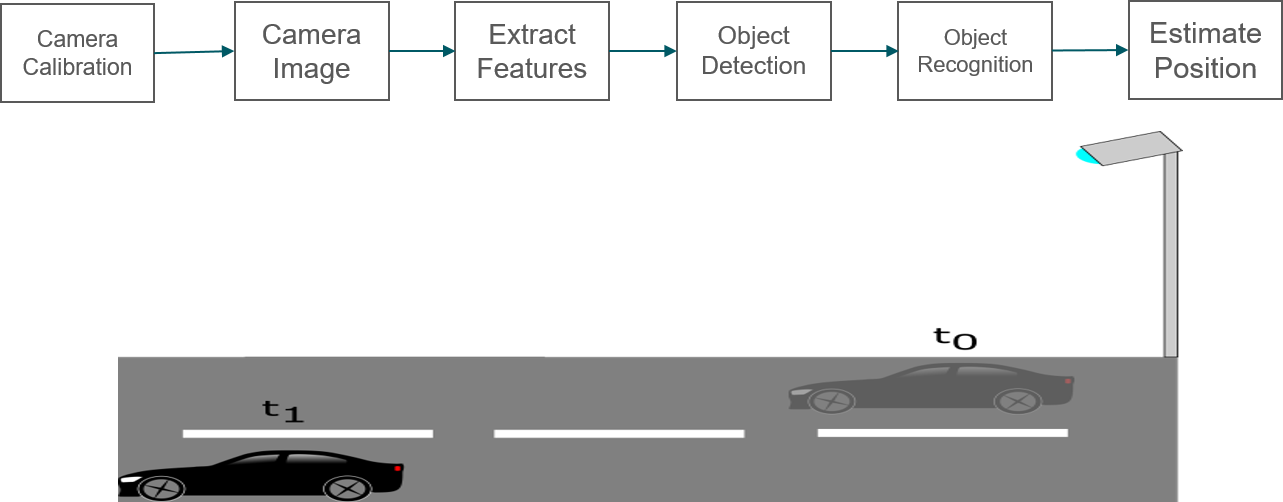
\includegraphics[width=\textwidth]{imagens/proposal1.png}
\caption{Proposal using only one camera with object calibration, this firts approach is based on \cite{8678911}}
\label{fig:proposal1}
\end{figure}


\subsection{Proposal 2 – One camera with known map}
\begin{figure}[H]
\centering
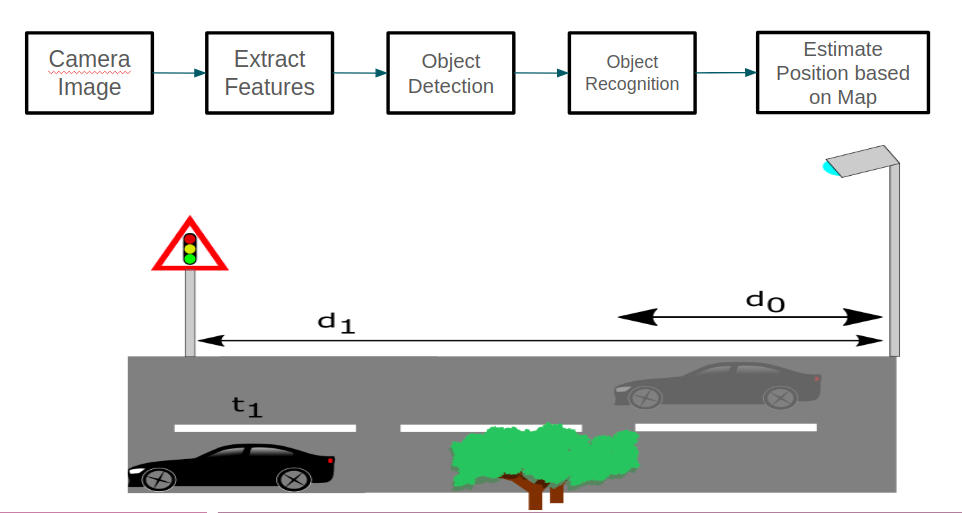
\includegraphics[width=\textwidth]{imagens/proposal2.png}
\caption{Proposal using Proposal 2 – One camera with known map}
\label{fig:proposal2}
\end{figure}


\subsection{Proposal 3 – Multicameras}
\begin{figure}[H]
\centering
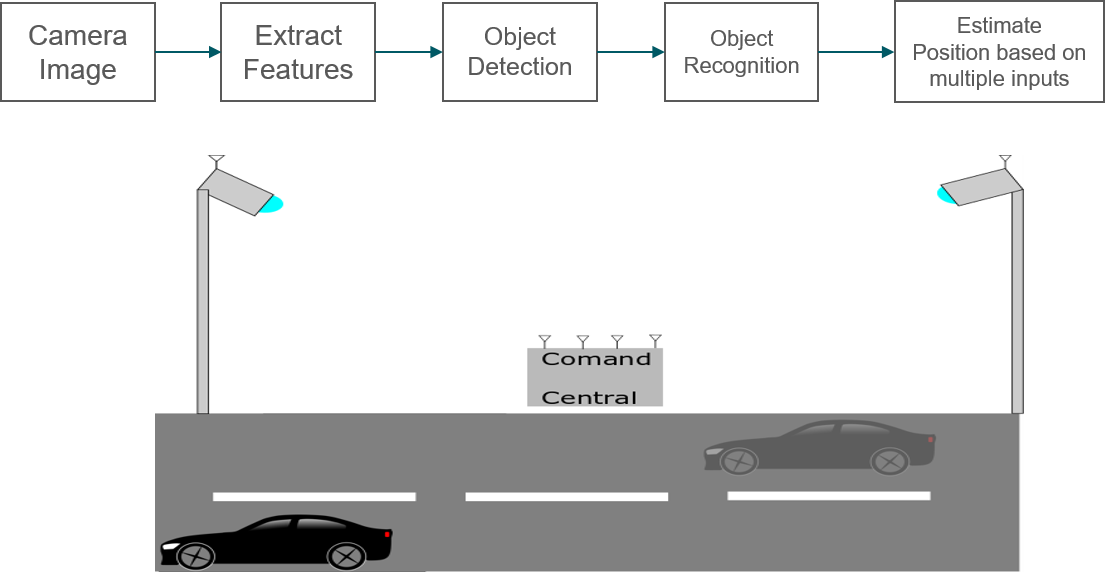
\includegraphics[width=\textwidth]{imagens/proposal3.png}
\caption{Proposal using multicameras}
\label{fig:proposal3}
\end{figure}



\section{Inverse Perspective Mapping }
Inverse perspective mapping is a mathematical technique that remove the effects of distortion of a picture when transforming the perspective of the image to another perspective. In spite of disparity mapping, inverse perspective mapping method requires only one camera and this method can't provide depth information directly ~\cite{Tuohy2010}.

Camera must be located in front of the car with an angle of \(\theta\) to down. Figure \ref{fig:ImageRelationSystem} shows the setup.

\begin{figure}[h]
\centering
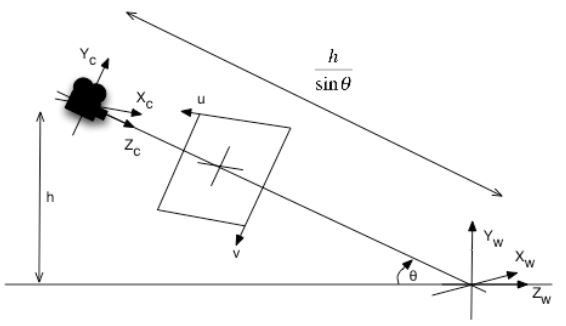
\includegraphics[scale=0.5]{imagens/Inverse Perspective Mapping.JPG}
\caption{Image coordinate system in relation to world coordinate
system.}
\label{fig:ImageRelationSystem}
\end{figure}
\par


This setup was selected based on solution of \cite{Wongsaree2018}, the mathematical background is to create top-down view, the surface road point is known as $(X_w,Y_w,Z_w)$
that projects to the image plane $(u,v)$ is a must. As disrupted in Figure \ref{fig:ImageRelationSystem}. For rotatation angle $(\theta)$, which is angle between camera and the surface, the IPM equation is based on \cite{7759904} and is shown is Equation \ref{eq:eq1}:

\begin{equation}
    (u,v,1)^T = K\cdot T \cdot K (X_w,Y_w, Z_w,1)^T
    \label{eq:eq1}
\end{equation}

where R is the rotation matrix given in the equation \ref{exp2}.
\begin{equation} \label{exp2}
R=
\begin{bmatrix}
1 & 0 & 0 & 0\\
0 & \cos{\theta} & -\sin{\theta} & 0\\
0 & \sin{\theta} & \cos{\theta} & 0\\
0 & 0 & 0 & 1
\end{bmatrix}
\end{equation}
\par

T is the translation matrix given in the equation \ref{exp3}. Where h means the height of the position of the camera.
\begin{equation} \label{exp3}
T=
\begin{bmatrix}
1 & 0 & 0 & 0\\
0 & 1 & 0 & 0\\
0 & 0 & 1 & \frac{-h}{\sin{\theta}}\\
0 & 0 & 0 & 1
\end{bmatrix}
\end{equation}


\par
K is the camera parameter matrix given in the Equation \ref{exp4}. Where $f$ is the focal length of the camera, $s$ is the skew parameter and $u_0, v_0$ are the center of the pixel of desired image size. 
\begin{equation} \label{exp4}
K =
\begin{bmatrix}
f & s & u_0 & 0\\
0 & f & v_0 & 0\\
0 & 0 & 1 & 0\\
\end{bmatrix}
\end{equation}

The Equation \ref{exp4} can be replaced using the real parameters of this test scenario and these parameters are $f = 2.92 mm, s=0, u_0=240, v_0=160$. Replacing the Equations \ref{exp2},\ref{exp3}, \ref{exp4} into the initial Equation \ref{eq:eq1}, achieving the new Equation \ref{eq:eq2}.

\begin{equation}
    \begin{bmatrix}
u\\ 
v\\ 
1
\end{bmatrix}
=\begin{bmatrix}
P_{11} & P_{12} & P_{13} & P_{14}\\ 
P_{21} & P_{22} & P_{23} & P_{24}\\ 
P_{31} & P_{32} & P_{33} & P_{34}
\end{bmatrix}
\begin{bmatrix}
X_w\\ 
Y_w\\ 
Z_w\\
1
\end{bmatrix}
\label{eq:eq2}
\end{equation}

where the matrix P was gotten from product between K, T, and R. As is only necessary to evaluate the position of the road, so the coordinate $Y_w$ can be equal to 0, so simplifying the Equation \ref{eq:eq2}, so it is given by Equation \ref{eq:eq3}.

\begin{equation}
    \label{eq:eq3}
    \begin{bmatrix}
u\\ 
v\\ 
1
\end{bmatrix}
=\begin{bmatrix}
P_{11} & P_{12}  & P_{14}\\ 
P_{21} & P_{22}  & P_{24}\\ 
P_{31} & P_{32}  & P_{34}
\end{bmatrix}
\begin{bmatrix}
X_w\\ 
Z_w\\
1
\end{bmatrix}
\end{equation}

Based on the Equations above, it is possible to infer the Equation \ref{eq:eq4} for compute the distance from the camera until the object. 

\begin{enumerate}
    \item Calculating average intensity in row direction from bottom row up to top row
    \item The average intensity of each row is compared with the threshold level (obtained from the experimental) which is 50. The starting position of an object is indicated if the average intensity in that row is greater than 50 and the order of that row is stored in a parameter p.
    \item The distance between object and vehicle is therefore calculated using a linear equation given in \ref{eq:eq4}.
\end{enumerate}

\begin{equation}
    \label{eq:eq4}
    d = ap+b
\end{equation}

where $d$ is distance between camera and object and vehicle in meter, $p$ is the order of the row that object is detected and $a, b$ are constants.

 
\section{Framework Architecture} 

\begin{figure}[H]
\centering
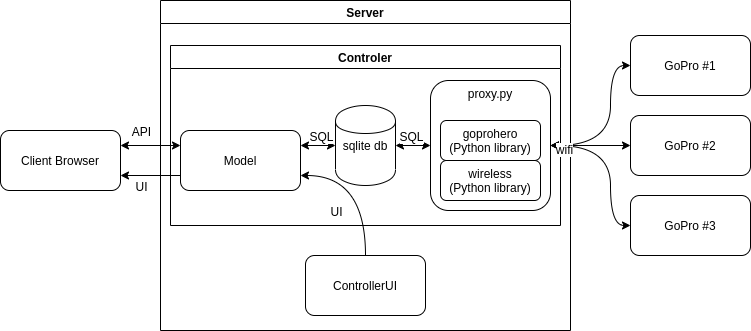
\includegraphics[scale=0.6]{imagens/diagram.png}
\caption{Architecture approach of framework}
\label{fig:framework}
\end{figure}

\begin{figure}[H]
\centering
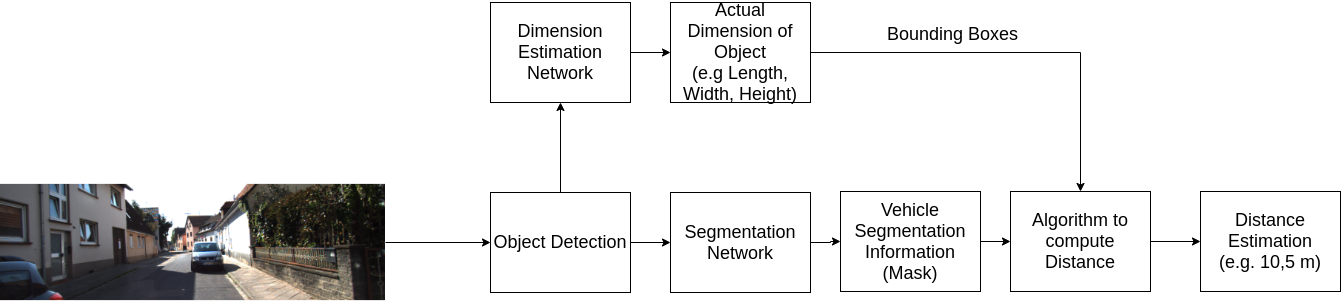
\includegraphics[width=\textwidth]{imagens/Network Behavior.png}
\caption{Architecture approach of framework}
\label{fig:networkBehavior}
\end{figure} 
	\chapter{Results}
\label{capitulo5}




\begin{figure}[H]
\centering
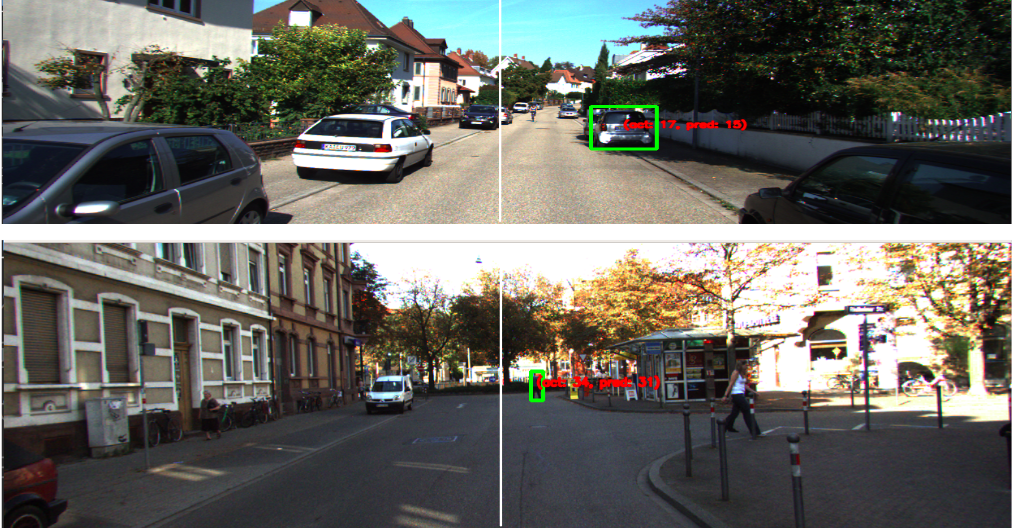
\includegraphics[width=\textwidth]{imagens/ouput.png}
\caption{Output results from framework using single stereo camera}
\label{fig:output}
\end{figure}


\section{Validation}

For validation purpose, it was used a commercial laser measurement as shown in Figure \ref{fig:laser_meas}, this model is known as Bosch DLE 40 Professional $^{\tiny{\textregistered}}$. 



\begin{figure}[H]
\centering
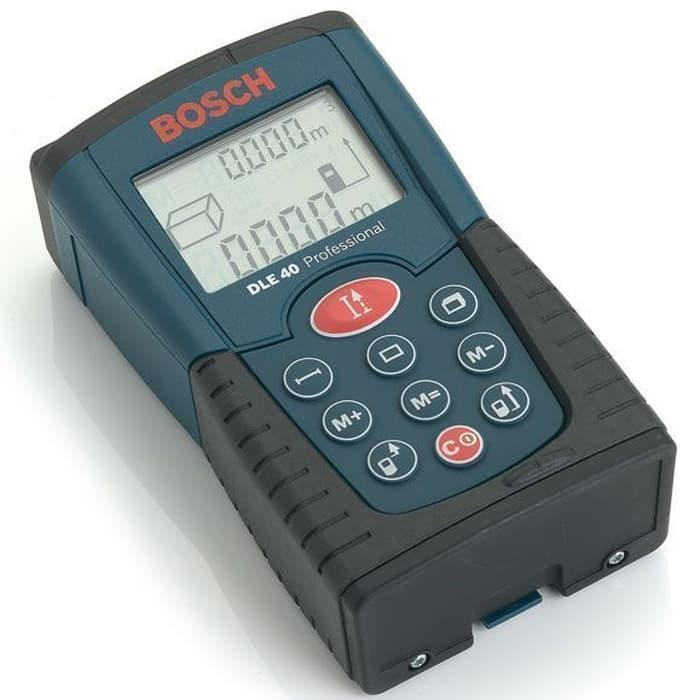
\includegraphics[scale=0.3]{imagens/trena.jpg}
\caption{Commercial laser measurer}
\label{fig:output}
\end{figure}

The instrumental error rate is $\pm 1.5 mm$, thereby we repeated the measure three times and computed the mean, and standard deviation as well. In Table \ref{tab:tab_measure} is shown the measurements with the camera positioned at $2.01$ m from the ground. And in the Figure \ref{fig:park} is shown the position of the cars along the parking lot. 



\begin{table}[H]
\centering
\caption{Measurements collected with a commercial measurer}
\begin{tabular}{l|l|l|l} 
\toprule
Car & First measure & Second measure & Third measure  \\
\#1   & 4.25          & 4.47           & 4.51           \\
\#2   & 11.01         & 11.21          & 11.11          \\
\#3   & 16.12         & 16.35          & 16.26          \\
\#4   & 19.63         & 19.69          & 19.66          \\
\#5   & 23.08         & 23.18          & 23.01          \\
\bottomrule
\end{tabular}
\label{tab:tab_measure}
\end{table} 



\begin{figure}[H]
\centering
\label{fig:park}
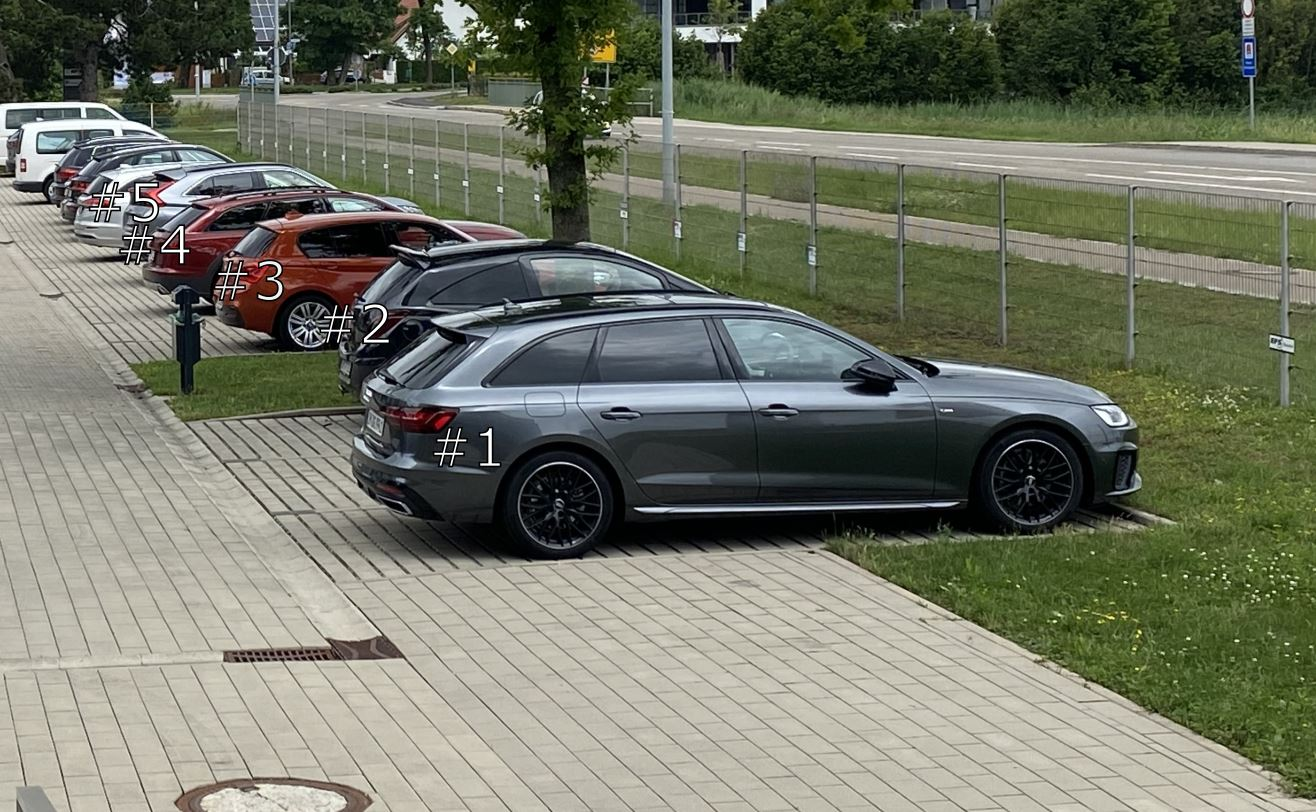
\includegraphics[scale=0.5]{imagens/park.JPG}
\caption{Position of the cars on the parking lot}
\label{fig:output}
\end{figure}
 
    \chapter{Conclusion}
\label{capitulo6}
% 	\bibliographystyle{apalike}	
    \nocite{*}
	\bibliographystyle{abnt-num} % estilo bibliográfico ABNT numérico
% 	\bibliographystyle{abnt-alf} % estilo bibliográfico ABNT alfabético
% 	\bibliographystyle{sbc}  % estilo bibliográfico da Sociedade Brasileira de Computação (SBC)
	
	%\renewcommand{\bibname}{REFERÊNCIAS BIBLIOGRÁFICAS} %Define o Caption da seção de bibliografia
	%\addcontentsline{toc}{chapter}{REFERÊNCIAS BIBLIOGRÁFICAS}
	
	%não pode ter espaço entre os nomes dos arquivos bib
	\bibliography{referencias}
	\appendix
	\chapter{Appendix}

\section{Code to control the app}]\label{ap:app}
\lstinputlisting[language=Python]{code/app.py}

\section{Code to detect the bounding boxex}\label{ap:bbox}
\lstinputlisting[language=Python]{code/bbox.py}

\section{Code to control the camera}\label{ap:camera}
\lstinputlisting[language=Python]{code/camera.py}

\section{Abstraction of Darknet in Pytorch}\label{ap:darknet}
\lstinputlisting[language=Python]{code/darknet.py}

\section{Code for data preprocessing}\label{ap:preprocess}
\lstinputlisting[language=Python]{code/preprocess.py}

\section{Base Template}\label{ap:template1}
\lstinputlisting[language=html]{code/base.html}

\section{Index Template}\label{ap:template2}
\lstinputlisting[language=html]{code/index.html}







\end{document}

